%   Filename    : chapter_2.tex 
\chapter{Review of Related Literature}
\label{sec:relatedlit}

This chapter discusses the features, capabilities, and limitations of existing research, algorithms, or software  that are related/similar to Ha.Zee. Ha.Zee, as an application, identfied the vehicles passing across the camera feed and calculates their $PM_{2.5}$ emission average


\begin{comment}
%
% IPR acknowledgement: the contents withis this comment are from Ethel Ong's slides on RRL.
%
Guide on Writing your RRL chapter
 
1. Identify the keywords with respect to your research
      One keyword = One document section
                Examples: 2.1 Story Generation Systems
			 2.2 Knowledge Representation

2.  Find references using these keywords

3.  For each of the references that you find,
        Check: Is it relevant to your research?
        Use their references to find more relevant works.

4. Identify a set of criteria for comparison.
       It will serve as a guide to help you focus on what to look for

5. Write a summary focusing on -
       What: A short description of the work
       How: A summary of the approach it utilized
       Findings: If applicable, provide the results
        Why: Relevance to your work

6. At the end of each section,  show a Table of Comparison of the related works 
   and your proposed project/system

\end{comment}

\section{Air Quality Monitoring Systems}
Air quality monitoring systems are systems that collect data to record and analyze atmospheric emission levels. There are various systems for air quality monitoring. Zoogman et al.\citeyear{zoogman_2017} showcased in the Journal of Quantitative Spectroscopy and Radiative Transfer, the use of satellite imagery for large-scale air quality monitoring. They call this instrument TEMPO (Tropospheric Emissions: Monitoring of Pollution), which collects data on tropospheric emissions such as \ch{NO2}, \ch{SO2}, \ch{H2CO}, Methane, etc. from a satellite in a geostationary orbit. TEMPO is wide-range and precise,  however, access to the equipment is limited.  A more accessible air monitoring system was made by Zheng et al. \citeyear{zheng_2016} using several sensors. This system makes use of low-power wide-area network (LPWAN) to give it a wider coverage compared to the IoT (Internet-of-Things ) and the air quality data can be accessed through a mobile application. These systems make use of dedicated sensors to collect emission data whereas this project will make use of computer vision and machine learning.


\section{Air Pollution from Vehicles}
The Philippines currently has a problem with air pollution. According to Tantengco \& Guinto \citeyear{TANTENGCO2022}, the Philippines’ $PM_{2.5}$ concentrations in urban areas exceed the WHO guideline value. They further state that the Philippines’ $PM_{2.5}$ levels reach $58.4 ug/m^{3}$ in traffic sites of Metro Manila during the dry season. Though there could be different sources of air pollution, 65 percent of the air pollutants come from mobile sources such as cars, motorcycles, trucks, and buses \cite{EMB_2015}. Not only can these mobile vehicles produce $PM_{2.5}$, they can also emit greenhouse gasses, which are just as harmful.

	\ch{CO2}, a component of greenhouse gasses, totaled “30 million tons and 56 thousand tons of particulate matter” \cite{FabianGota2009} in the Philippines and the transport sector contributed to 38 percent of fuel combustion back in 2000. The authors have noted that the motorized vehicle count would double by 2020. The increase in motorized vehicles also means an increase in their air pollution contribution. 

A study by Lu \citeyear{lu_2022} analyzes the emissions of vehicles due to their impact on air pollution and road-environmental safety. The results show that from 2018 to 2019, two hundred eighty-two vehicle emission standard violations were recorded by the Land Transportation Organization (LTO) office. All of these violations were due to smoke-belching from vehicles. Another result to note was that all the violations were during work hours (6:00 AM to 5:00 PM). The vehicles caught for dangerous emissions were more than 10 years old, with one-third between 10 to 19 years old. The paper concluded that not only ensuring safe vehicle emissions can play an important role in reducing air pollution, there is a need for implementation and monitoring of said vehicle emissions to be within a safer threshold. The researcher notes that the Philippines still needs improvement in addressing the concerns of vehicles contributing to air pollution. Finding a way to quantify and monitor these emissions can be a step towards reaching said 'safer threshold' of air quality.

A recent paper by \citeA{rito_lopez_biona_2021} raises the concern of quantifying traffic flow, which in this context, is also used for calculating the emission and energy consumption factors. The researchers state that calculating traffic flow has other researchers “deal with complex and arduous tasks, especially when conducting actual surveys”. In this paper, the researchers instead utilized crowdsourced data from Google Maps to estimate mobile emissions and energy use from the traffic flow of the road. The method was used on the EDSA highway in the Philippines and managed to garner an 8.63\% error concerning the total vehicle count.

\section{Vehicle Detection and Tracking}

	Vehicle detection is a method of identifying a vehicle via a camera. Research on this method started being conducted during the late 1970s \cite{NathDeb2012} and as more vehicles enter our roads, there has also been more interest in the topic. Meng et al. \citeyear{Meng_2020} defined vehicle detection-based computer vision as aiming at identifying and locating vehicles through digital images or videos. They further simplify the idea by stating that vehicle detection detects “blocks”, which reflect the vehicle’s position from the images and videos.

	A similar paper by Yang et al. \citeyear{yang_2020} proposed an “object tracker–detector combined with an object tracking algorithm” for tracking vehicles in traffic. They created the tracker by combining strategies for the You Only Look Once (YOLO) model (which will be talked about in section 2.4) with a correlation filter (CF) tracker. To elaborate on object detection, a detection box merge strategy was used for YOLO. This is to prevent the algorithm from partially detecting an object or detecting it more than once. For the tracker, a “deep feature-based CF tracker” was designed. Lastly, to combine both into a tracker-detection program, a tracker was “first used to predict the location of an object in the subsequent frame.”

	Another process to detect and track the vehicle would be through background subtraction. Background subtraction, according to Huang BJ. et al. \citeyear{Huang_2017}, is used to extract moving objects and then filter unwanted images through image processing tools. 
	
	Moreover, another method of vehicle detection and recognition – via infrared image and feature extraction was recently studied by Li et al. \citeyear{li_2022}.
	The paper states that due to infrared images having shortcomings such as poor contrast or blurred edges, they mainly studied the color space preprocessing of the image with the use of the threshold segmentation method and infrared image enhancement to separate the vehicle and the background. Techniques such as the median filter and the improved histogram equalization are then used to remove the noise from the infrared image and to enhance the contrast of the image, respectively. The vertical Sobel operator is then selected to enhance the vertical edge of the image. The vertical Sobel operator is used to enhance the vertical edge of the image. Lastly, vertical edge symmetry, aspect ratio, and gray-scale symmetry are utilized for vehicle detection and recognition.


\section{Object Detection Algorithms}
Object detection in the context of this study, involves detecting an instance/instances of objects from one or several image classes \cite{Amit_Felzenszwalb_Girshick_2020}. The same researchers state that object detection systems construct a model for object class via a “training example set”. The following are some algorithms utilized in constructing object detection models:

\subsection{YOLOv5}

Yolov5 is a pre-trained algorithm that uses a system of grids to detect objects from images or videos (https://docs.ultralytics.com/). 
One application of this algorithm was done by Yan et al. \citeyear{yan_2021} for an apple-picking robot. YOLOv5 was used to identify apples, however, the algorithm cannot detect apples that are safe to pick and those that are not. This may cause the picking arm of the robot to break if it tries to grasp an apple that is occluded by a solid object. They solved this problem by improving on the modules used for the algorithm. This is not a problem for this project as it only counts the number of vehicles without interacting with them. 

In a study done by Zhou et al. \citeyear{zhou_2021}, they applied YOLOv5 algorithm to detect safety helmets on workers. The algorithm had an average detection speed of 110 fps in real time. The model, which was trained and tested using 6045 data sets, proved to be viable for real-time detection with a 94.7\% effectiveness.


\subsubsection{YOLOv5 Architecture}
The YOLOv5, alongside other YOLO algorithms, is a single-stage detector and is composed of three fundamental components: the backbone, the neck, and the tail \cite{Solawetz_2020}. shown in Figure \ref{fig:yolo_archi} is the graphical representation of the architecture, which was from the YOLOv4 study by Bochkovskiy et al. \citeyear{Bochkovskiy_Wang_Liao_2020}.

\begin{figure}[!htbp]
	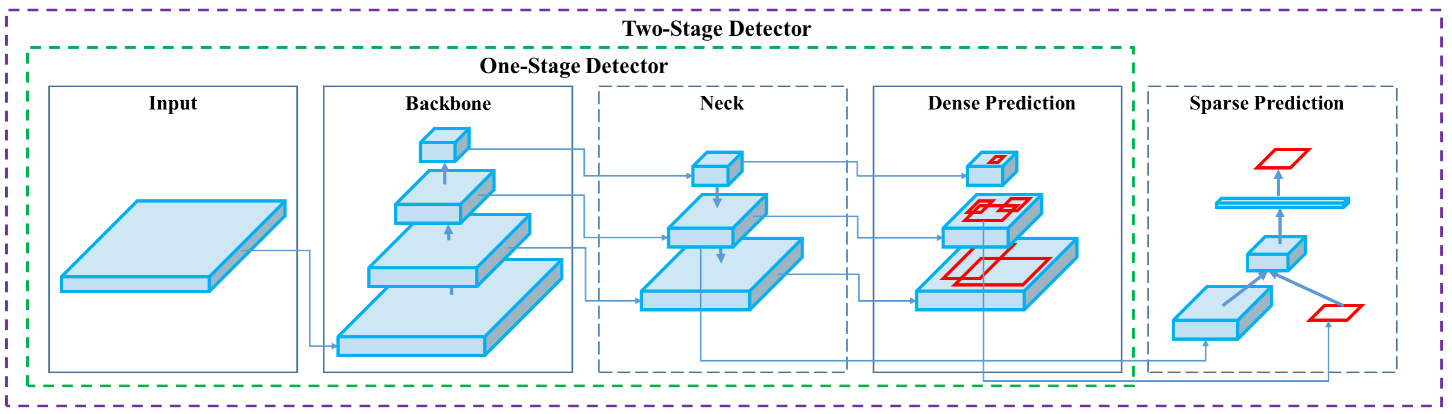
\includegraphics[width=\linewidth]{yolo_arci.png}
	\caption{Graphical depiction of the architecture of the YOLO algorithms}
	\label{fig:yolo_archi}
\end{figure}
\FloatBarrier


The primary function of a detection model's backbone is to extract crucial features across various resolutions, capturing relevant information about object position and structure \cite{Kateb_2021}. The CSP (Cross-Stage Partial) Bottleneck is employed in YOLOv5 to assemble image features. The CSP architecture resolves the issue of redundant gradient computations found in larger ConvNet backbones, leading to reduced parameters and computational operations (FLOPS) while maintaining comparable importance, which holds significant value for the YOLO family of models, as it prioritizes both inference speed and compact model size as crucial factors \cite{Solawetz_2020}. YOLOV5 uses the CSP-Darknet53 which is a modified version of previous algorithms \cite{Jocher_Waxmann_2023}.

The neck component constructs feature pyramids which are essential for enabling the model to detect objects of varying sizes. Additionally, the neck acts as a bridge, connecting the backbone to the head component. In YOLOv5, two specific structures are utilized within the neck component to facilitate these functionalities: SPPF (Spatial Pyramid Pooling Fusion) and New CSP-PAN (Cross-Stage Partial - Path Aggregation Network)  \cite{Jocher_Waxmann_2023}.

Finally, the head component employs the YOLOv3 Head to make the final predictions of bounding boxes and class scores  \cite{Jocher_Waxmann_2023}.

\subsection{Region-based Convolutional Neural Networks}

Region-based Convolutional Neural Networks or R-CNN, is a technique that uses Neural networks to detect objects; this algorithm requires a hefty processing time \cite{Cuong_Trinh_Meesad_Nguyen_2022}. The researchers of that study further mention the “area suggestions”, which is an image that is extracted into small dimensions and used as inputs to the R-CNN model. The R-CNN model then uses a selective search method to extract reference ranges, then the areas are divided into a set of objects, followed by selective searching to provide candidates suggestions. Once finished, these ‘proposals’ are sent to the cumulative Neural Network (CNN)  and a Support Vector Machine (SVM) is used to classify the presence of an object.

In a study done by Rafique et al. \citeyear{Rafique_Pedrycz_Jeon_2017}, they utilized the R-CNN, along with its successors: Fast-RCNN and Faster-RCNN, to provide solutions for detecting vehicle license plates. It was used with the goal of license plate detection in every frame of a video, detection of partial or obscured license plates, and the detection of license plates whilst using a moving camera on moving vehicles.



\section{Vehicle Recognition/Identification Applications}
	
	In this study, Vehicle Recognition or Identification Applications would be considered as applications that either use any form of video-based software in locating the vehicle on the display feed; or software where static images can be used in identification. Chintalacheruvu and Muthukumar \citeyear{chintalacheruvu_2012} state that video-based vehicle detection technology has features such as: “non-intrusiveness and comprehensive vehicle behavior data collection capabilities”, and that it has become an integral part of f Intelligent Transportation System (ITS)

	V-App Vehicle Detection is a real-time vehicle detection system that utilizes the visual analytics provided by Meraki Smart Cameras and a License Plate Recognition function to ‘overcome the limitations of common sensors’. It also has features such as vehicle distribution, which detects transit vehicles in an area by grouping them into categories; vehicle count and directions, which gets info on the total amount of vehicles transited and their direction details; and average busiest hours, which shows the higher transit and occupancy peaks in a graph \cite{VAPP_ND}.

	BitRefine Heads is a computer vision platform that “utilizes deep learning algorithms to perform high-level visual analysis”. It is a platform that detects everyday objects from any angle and also has a vehicle detection system. The recognition module is pre-trained and can detect vehicles as well as recognize the car’s model based on the visual features. It gets its video source from an Real Time Streaming Protocol (RTSP) stream from an IP camera. The video then goes to a neural classifier that locates the vehicle in the frame and identifies its class using its own vehicle recognition module’s database.  The tracking module then takes the results and builds the vehicle’s movement track. Then it passes additional images of said vehicle to the neural module to check whether the class is correct \cite{BITREFINE_ND}.


\section{Vehicle Emission Calculator Applications}
	In this study, a vehicle emission calculator application would be regarded as an application that provides the total emission count or estimate of a vehicle after given inputs such as: vehicle type, vehicle make and model, fuel type, and the like.
	
	The $PM_{2.5}$ Footprint Calculator v1.01 is an online web browser tool by the constituents of Mahidol University, Thailand. It calculates the primary and secondary $PM_{2.5}$ emissions ($PM_{2.5}$, \ch{N2O}, \ch{NH3}, and \ch{SO2}) by asking for the distance traveled, age of the vehicle, fuel type, and city location. Due to the calculator being “developed as a tool for enhancing environmentally sustainable passenger transport in Thailand,” it also displays information that assesses the health costs of health impacts of a vehicle. The effect of the emissions on humans’ health is calculated using  Disability-Adjusted Life Years (DALY) – which, according to the World Health Organization \citeyear{WHO_nd}, One DALY represents the loss of the equivalent of one year of full health. The calculator is divided into different vehicle types, each having its dedicated page for calculating the $PM_{2.5}$ levels \cite{pm25_footprint}.
	
	

	The Myclimate Car calculator is an online web browser application that determines the \ch{CO2} emissions of a car during its travel. The application asks for the distance traveled, along with the fuel type and fuel consumption. Users also have the option to enter the cart type (compact, mid-range, luxury/SUV/Van) to add to the calculation of the \ch{CO2} amount.  The basis of this calculation is through the utilization of the ecoinvent database (Version 3.6), using the IPCC 2013  (Intergovernmental Panel on Climate Change) evaluation method. The emissions are calculated per vehicle kilometer (vkm). The application creators further note that there is an uncertainty margin of 5\% added to the emissions due to statistical values used in the calculations \cite{MCF_ND}.

	The Next Greencar Make/Model Search Tool is an online car make and model search tool by Nextgreencar.com, a website established in 2007 to help car buyers transition from “fossil cars” to electric cars. This search tool takes the input of a car’s manufacturer and/or a specific model to provide results of: tail-pipe \ch{CO2}, \ch{N2O}, particulate emissions, and the NGC Rating. NGC Rating or Next Green Car Rating is a rating developed by the company to assess the environmental impact \cite{Lilly_ND}.  The site then lists all the cars that satisfy the query, allowing users to compare them between their emissions. 

	The aforementioned applications use different techniques to calculate the harmful emissions from different vehicles but they commonly share the same process of asking for input: from the user via typing in the required information to output the estimated $PM_{2.5}$, \ch{CO2}, \ch{N2O}, etc. emissions. Ha.Zee, while utilizing the same process of using predetermined pollutant levels being assigned to a vehicle, relied on computer vision training instead of user input to determine the vehicle and estimate the amount of the pollutant they would emit.

\section{Summary}
 As the usage of vehicles in the Philippines rapidly increases through the years, it also starts becoming the main contributor to air pollution in the country – a problem that the Philippines is still trying to mitigate. The aforementioned studies discern that in an attempt to solve this concern, emissions such as fine particulate matter ($PM_{2.5}$) and greenhouse gases (\ch{CH4}, \ch{N2O}, and \ch{CO2}) from mobile vehicles are collected and analyzed by making applications that can either calculate or keep track of the pollutant emissions. It is notable that most of the related applications cited as related literature are focused on manual input from the user. As these calculators use vehicle types to calculate estimates, the researchers sought out emerging technologies that use similar strategies in identifying vehicles.
 
	Computer vision and machine learning are new technologies that have been utilized for the benefit of identifying objects. This also means that vehicles and their types are subjects that can be identified by these technologies. Some of the applications used as an example can not only identify vehicles from a live video feed, but also produce results that list the vehicle's type. In addition, The related literature show that there is interest in the field and that different algorithms such as YOLO and R-CNN are constantly being developed for improvement of object detection.
	
	As aforementioned, object detection can be utilized for vehicle detection and identification of their types. The researchers thought of this strategy as a viable alternative to the calculators' need for manual user input. With the conceptualization of Ha.Zee, the idea of not needing user input to find pollution estimates was one of the main goals. While most of the related applications for vehicle tracking are viable options for the development of the system, they use an in-house system that is not publicly available to use without having to pay for them. The researchers instead opted to use YOLOv5, an open-source pre-trained algorithm that uses a system of grids to detect objects from images or videos to be used in the study. This information, along with the related studies of estimating pollutant emissions from vehicles, were used to support the researchers’ purposes of developing Ha.Zee.



